\chapter{Giao diện người dùng}
\label{chap:ui}

Pipeline dữ liệu chỉ có giá trị khi kết quả của nó đến được tay người dùng. Chương này trình bày ứng dụng web phục vụ năm nhóm người dùng: người học, giảng viên, cố vấn học tập, quản trị viên tổ chức và đội vận hành nền tảng dữ liệu.

\section{Quy trình thiết kế}

Phiên bản đầu của ứng dụng web là một bảng điều khiển demo hướng tới nhà phát triển: các nút giả lập sự kiện, mã định danh thô và ô nhập token nằm lẫn với kết quả. Nhóm thiết kế lại theo hai bước:
\begin{enumerate}
  \item \textbf{Mockup HTML tương tác} (\code{docs/ui-mockup/edu-platform-ui-mockup.html}): một file độc lập, dùng dữ liệu mẫu nhưng tuân theo đúng các quy tắc nghiệp vụ thật (điểm rủi ro 35/30/20/15, ngưỡng 30/60/80, $k = 5$, tỷ lệ giảm 30\%). Mockup giúp thống nhất bố cục và nội dung trước khi viết mã.
  \item \textbf{Hiện thực bằng React 18 + TypeScript} trong \code{apps/web}, giữ nguyên Vite, không thêm thư viện giao diện hay biểu đồ. Mọi màn hình đọc API thật. Những phần của mockup không có API tương ứng (độ tươi của báo cáo, kết quả kiểm tra chất lượng, ghi chú can thiệp) được bỏ ra thay vì dùng dữ liệu giả.
\end{enumerate}

\begin{figure}[H]
\centering
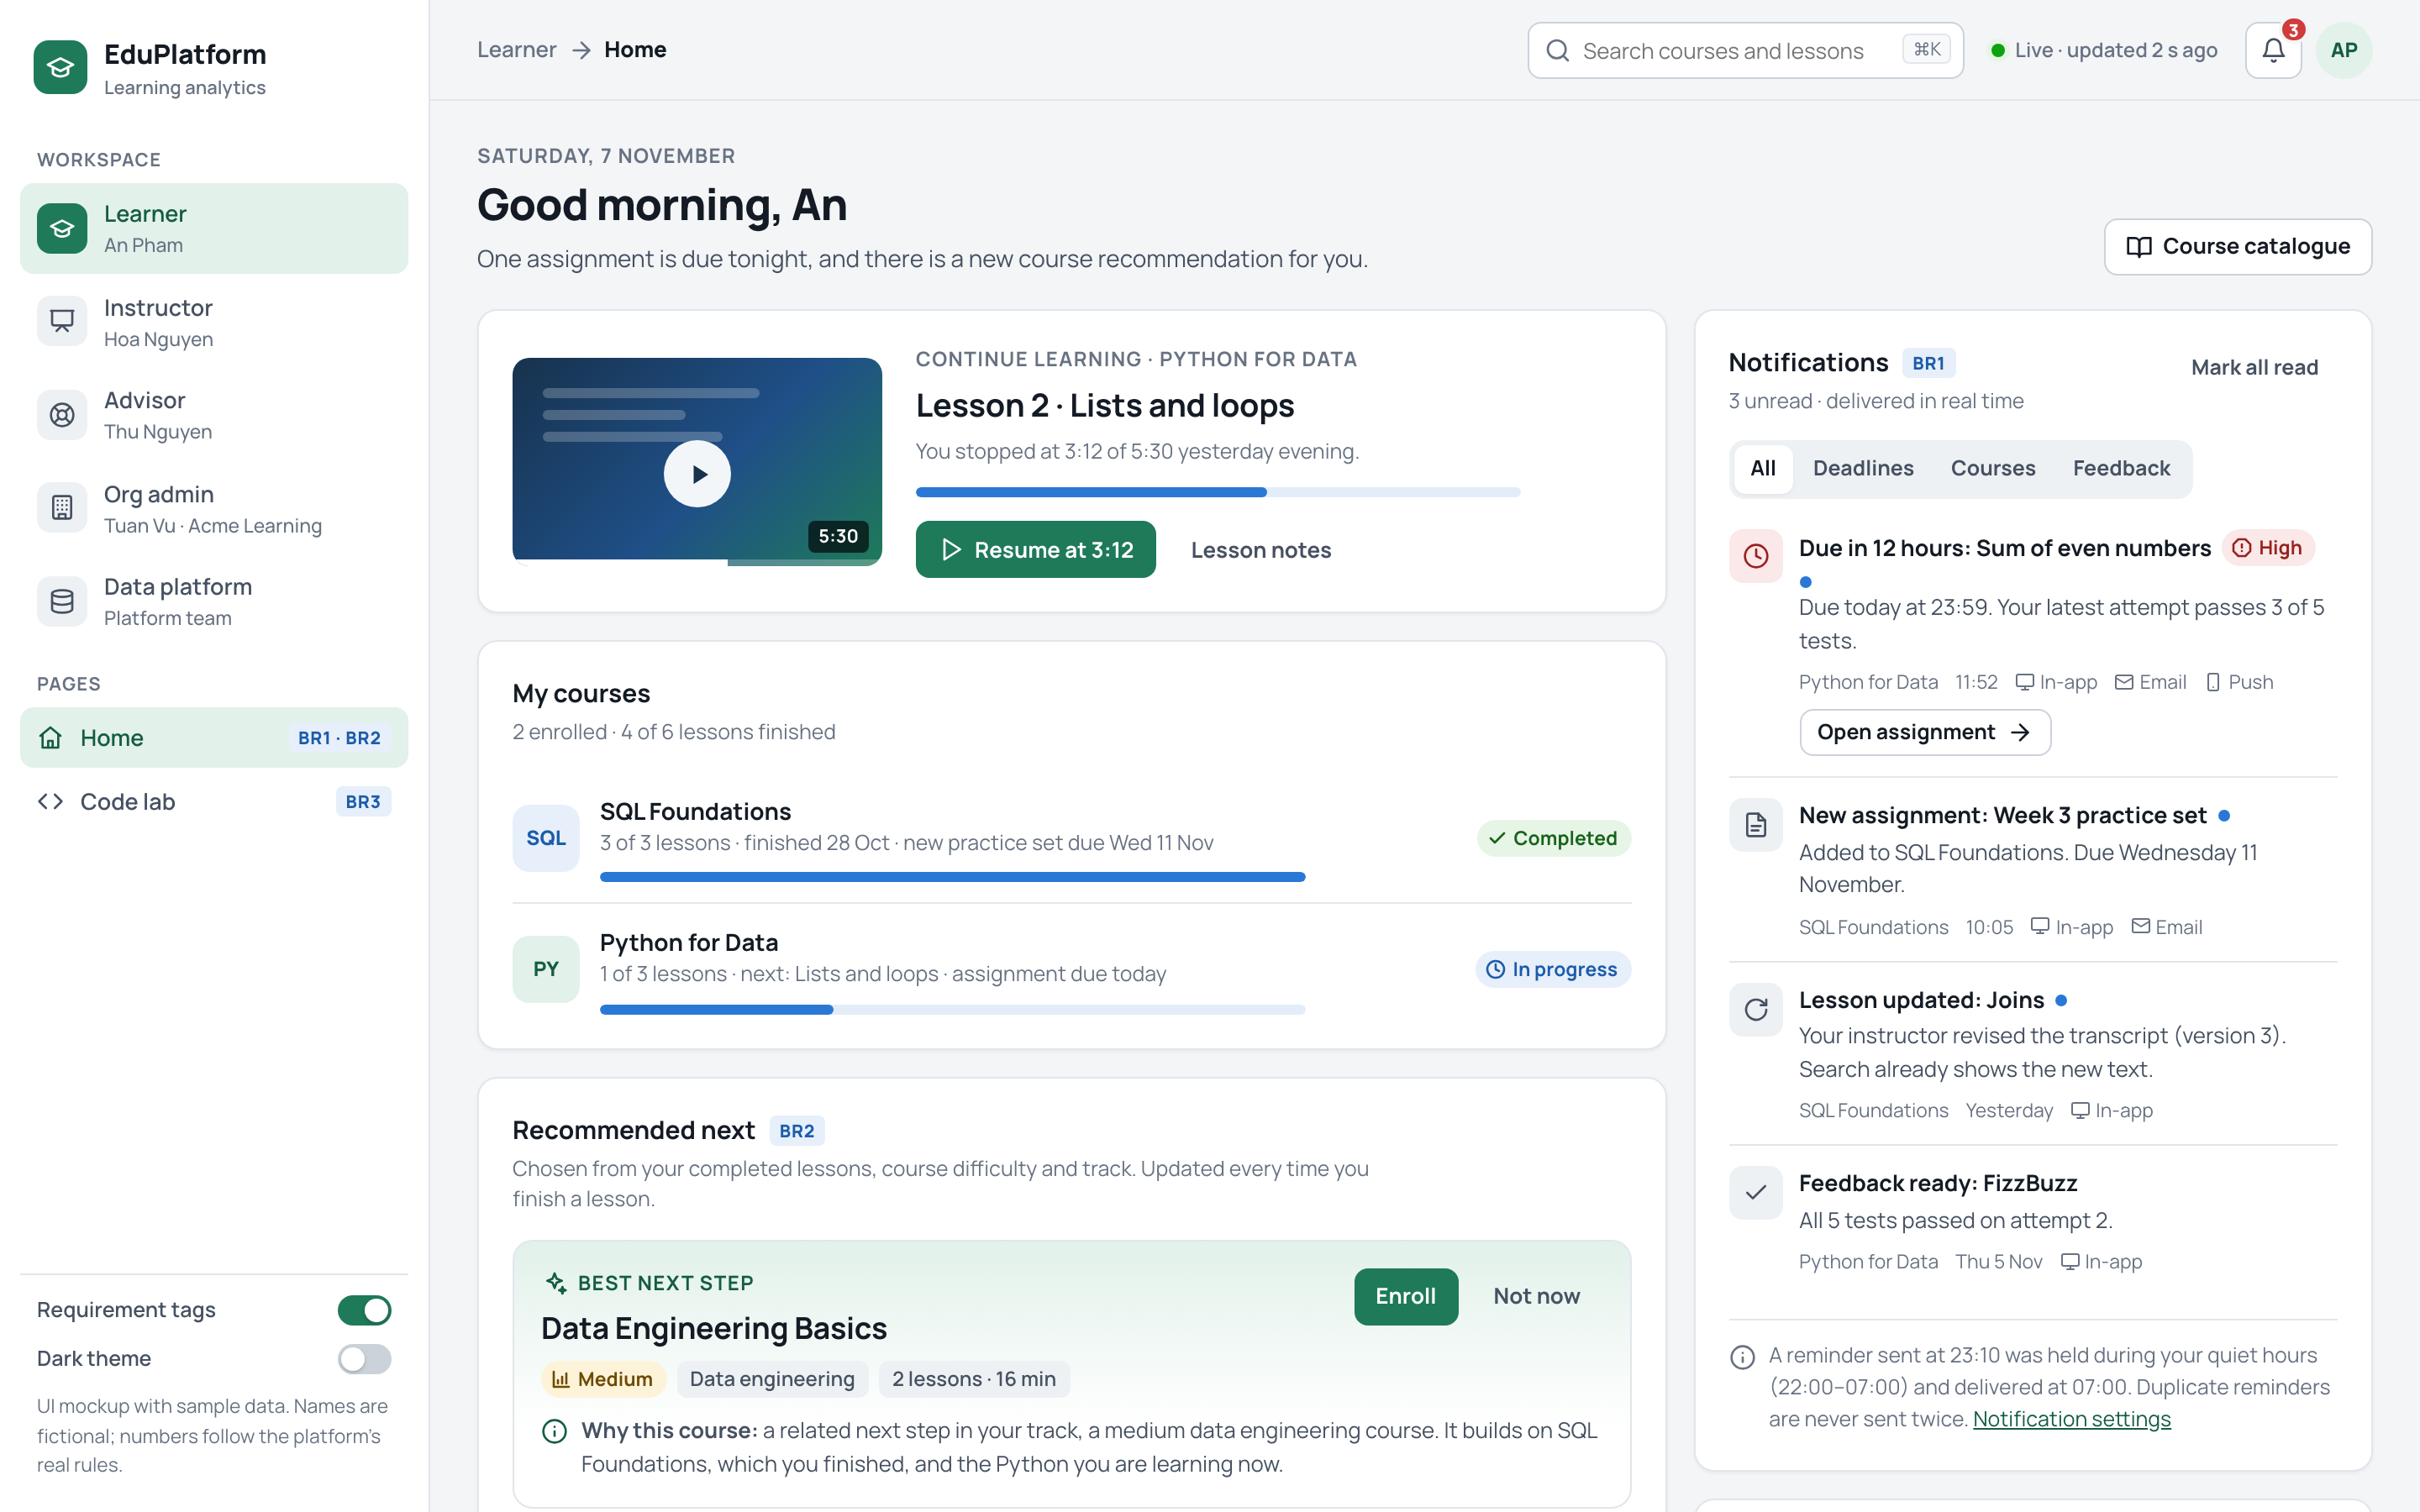
\includegraphics[width=\textwidth]{figures/mockup/learner-home.png}
\caption{Mockup: trang chủ người học với thông báo (BR1) và gợi ý khoá học kèm lý do (BR2)}
\label{fig:mock-learner}
\end{figure}

\section{Hệ thống thiết kế}

\begin{itemize}
  \item \textbf{Token thiết kế} cho màu, khoảng cách, bo góc và bóng đổ, có bộ giá trị riêng cho chế độ sáng và tối. Người dùng chuyển chế độ bằng một công tắc; mặc định theo hệ điều hành.
  \item \textbf{Bảng màu biểu đồ đã kiểm định}: màu phân loại theo thứ tự cố định và một dải màu xanh đơn sắc cho độ lớn (heatmap), đã kiểm tra khả năng phân biệt với người mù màu. Màu trạng thái (tốt, cảnh báo, nghiêm trọng, nguy hiểm) chỉ dùng cho trạng thái và luôn đi kèm biểu tượng và nhãn chữ, không bao giờ chỉ dựa vào màu.
  \item \textbf{Khả năng tiếp cận}: mọi biểu đồ có tooltip khi rê chuột và một bảng dữ liệu ``Xem dạng bảng'' thay thế; các nút có nhãn cho trình đọc màn hình; bố cục co giãn tới màn hình điện thoại mà không phải cuộn ngang.
  \item \textbf{Nhãn yêu cầu}: mỗi trang và mỗi khối được gắn nhãn BR tương ứng (có thể tắt). Nhãn này giúp truy vết từ giao diện về yêu cầu khi trình bày.
\end{itemize}

\section{Kiến trúc frontend}

Ứng dụng tổ chức theo \emph{không gian làm việc} (workspace), mỗi nhóm người dùng một workspace, chọn ở thanh bên (Bảng~\ref{tab:routes}). Thanh trên cùng có chỉ báo sự kiện trực tiếp (Server-Sent Events), thông báo của người học và trạng thái đăng nhập.

{\small
\begin{longtable}{@{}L{2.4cm}L{4.4cm}L{6.4cm}L{1.4cm}@{}}
\caption{Workspace, đường dẫn và trang}\label{tab:routes}\\
\toprule
\textbf{Workspace} & \textbf{Đường dẫn} & \textbf{Nội dung} & \textbf{BR} \\
\midrule
\endfirsthead
\toprule
\textbf{Workspace} & \textbf{Đường dẫn} & \textbf{Nội dung} & \textbf{BR} \\
\midrule
\endhead
Learner & \code{/learner} & Khoá học, gợi ý, phản hồi gần đây, thông báo & 1, 2 \\
Learner & \code{/learner/code-lab} & Trình soạn mã, phản hồi từng test, các lần nộp & 3 \\
Instructor & \code{/instructor/assessments} & Câu hỏi và chi tiết test case & 4 \\
Instructor & \code{/instructor/videos} & Heatmap theo phiên bản, lớp phủ hôm nay, thời điểm cần xem lại & 7 \\
Instructor & \code{/instructor/engagement} & Trung bình khoá học, học viên đang giảm & 8 \\
Instructor & \code{/instructor/content} & Xuất bản phiên bản, theo dõi đồng bộ, xem trước tìm kiếm & 8 \\
Advisor & \code{/advisor} & Hàng đợi rủi ro, phân rã điểm, lịch sử, cảnh báo & 5 \\
Org admin & \code{/admin} & Tiến độ tổ chức có ẩn nhóm nhỏ, xuất CSV & 6 \\
Data platform & \code{/pipeline} & Bộ đếm luồng, thông lượng, topic, DLQ, silver & -- \\
\bottomrule
\end{longtable}}

Các workspace Instructor, Advisor và Org admin được bảo vệ bằng một thẻ đăng nhập nhận token của vai trò. Token được giữ trong phiên của tab trình duyệt và dùng chung cho mọi trang của workspace. Máy chủ tự ánh xạ token sang danh tính, vai trò và phạm vi khoá học hoặc tổ chức; giao diện không tự khai báo quyền. Các điều khiển chỉ dành cho demo (giả lập sự kiện LMS, bộ sinh telemetry) được tách vào các khối ``Demo controls'' viền nét đứt. Biểu đồ được vẽ bằng SVG thuần với chiều rộng thật của phần tử, nên chữ không bị co giãn.

\section{Các màn hình chính}

Các ảnh trong mục này được chụp từ ứng dụng thật chạy trên dữ liệu của hệ thống (chế độ tối), trừ khi ghi là mockup.

\begin{figure}[H]
\centering
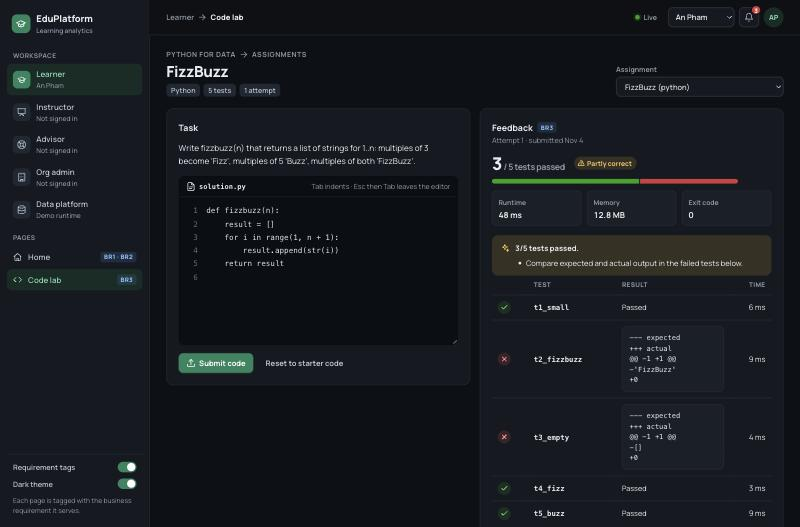
\includegraphics[width=\textwidth]{figures/ui/code-lab.jpg}
\caption{Code lab (BR3): bài nộp FizzBuzz được chấm trong sandbox, phản hồi từng test kèm diff}
\label{fig:ui-codelab}
\end{figure}

\begin{figure}[H]
\centering
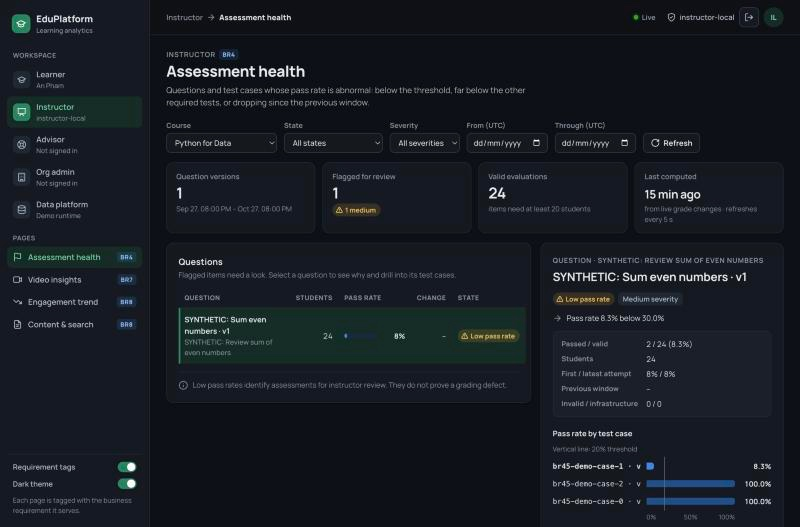
\includegraphics[width=\textwidth]{figures/ui/assessment-health.jpg}
\caption{Assessment health (BR4): câu hỏi bị gắn cờ và tỷ lệ đạt theo từng test case so với ngưỡng 20\%}
\label{fig:ui-br4}
\end{figure}

\begin{figure}[H]
\centering
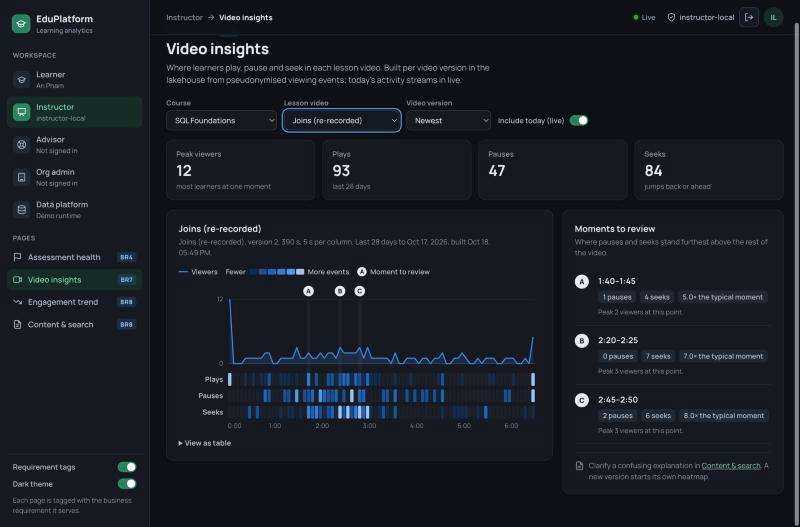
\includegraphics[width=\textwidth]{figures/ui/video-insights.jpg}
\caption{Video insights (BR7): heatmap play/pause/seek của phiên bản 2 video ``Joins'' (390 giây), kèm các thời điểm cần xem lại}
\label{fig:ui-br7}
\end{figure}

\begin{figure}[H]
\centering
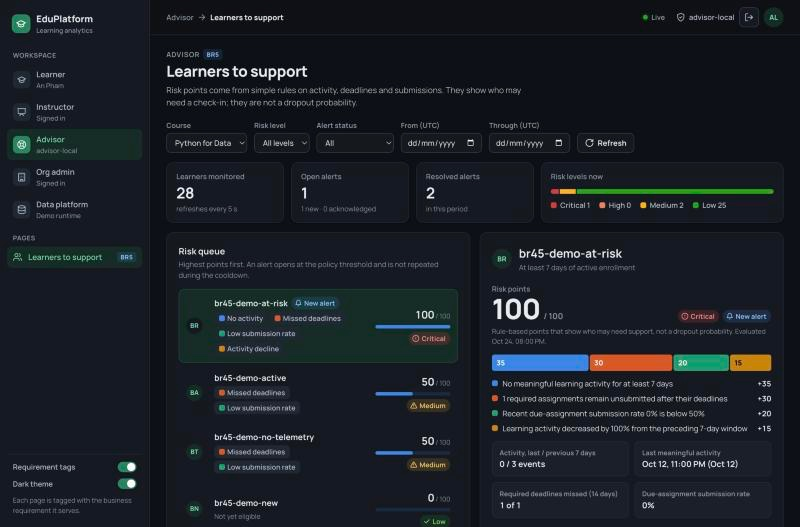
\includegraphics[width=\textwidth]{figures/ui/advisor.jpg}
\caption{Learners to support (BR5): hàng đợi rủi ro và phân rã 100 điểm thành 35 + 30 + 20 + 15}
\label{fig:ui-br5}
\end{figure}

\begin{figure}[H]
\centering
\begin{subfigure}{0.86\textwidth}
  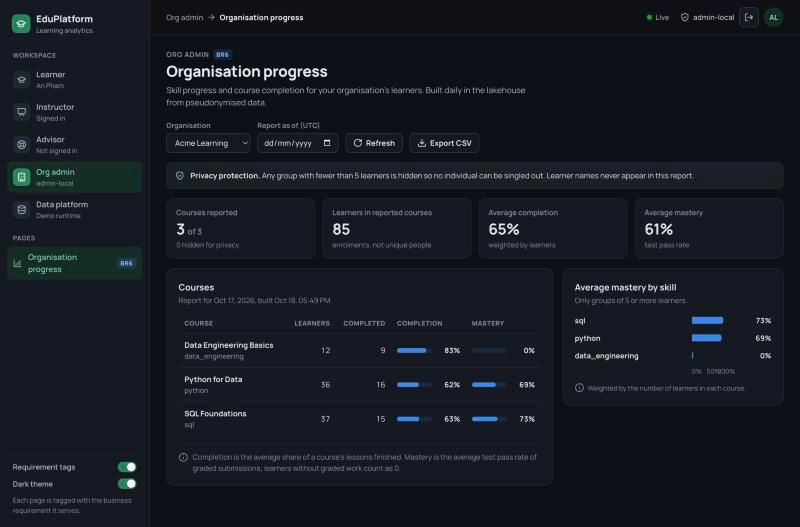
\includegraphics[width=\textwidth]{figures/ui/admin-acme.jpg}
  \caption{Acme Learning: mọi nhóm đủ 5 người nên được báo cáo}
\end{subfigure}\\[6pt]
\begin{subfigure}{0.86\textwidth}
  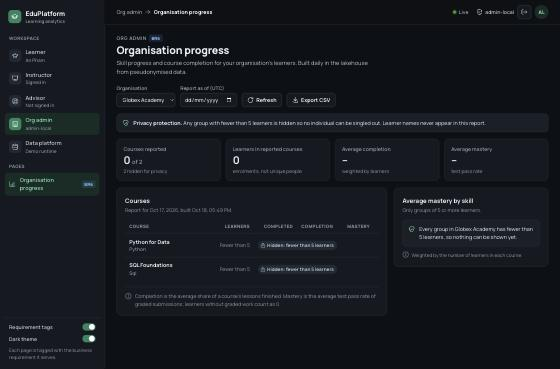
\includegraphics[width=\textwidth]{figures/ui/admin-globex.jpg}
  \caption{Globex Academy: mọi nhóm dưới 5 người nên bị ẩn, không lộ tỷ lệ hay quy mô chính xác}
\end{subfigure}
\caption{Organisation progress (BR6): k-anonymity với $k = 5$}
\label{fig:ui-br6}
\end{figure}

\begin{figure}[H]
\centering
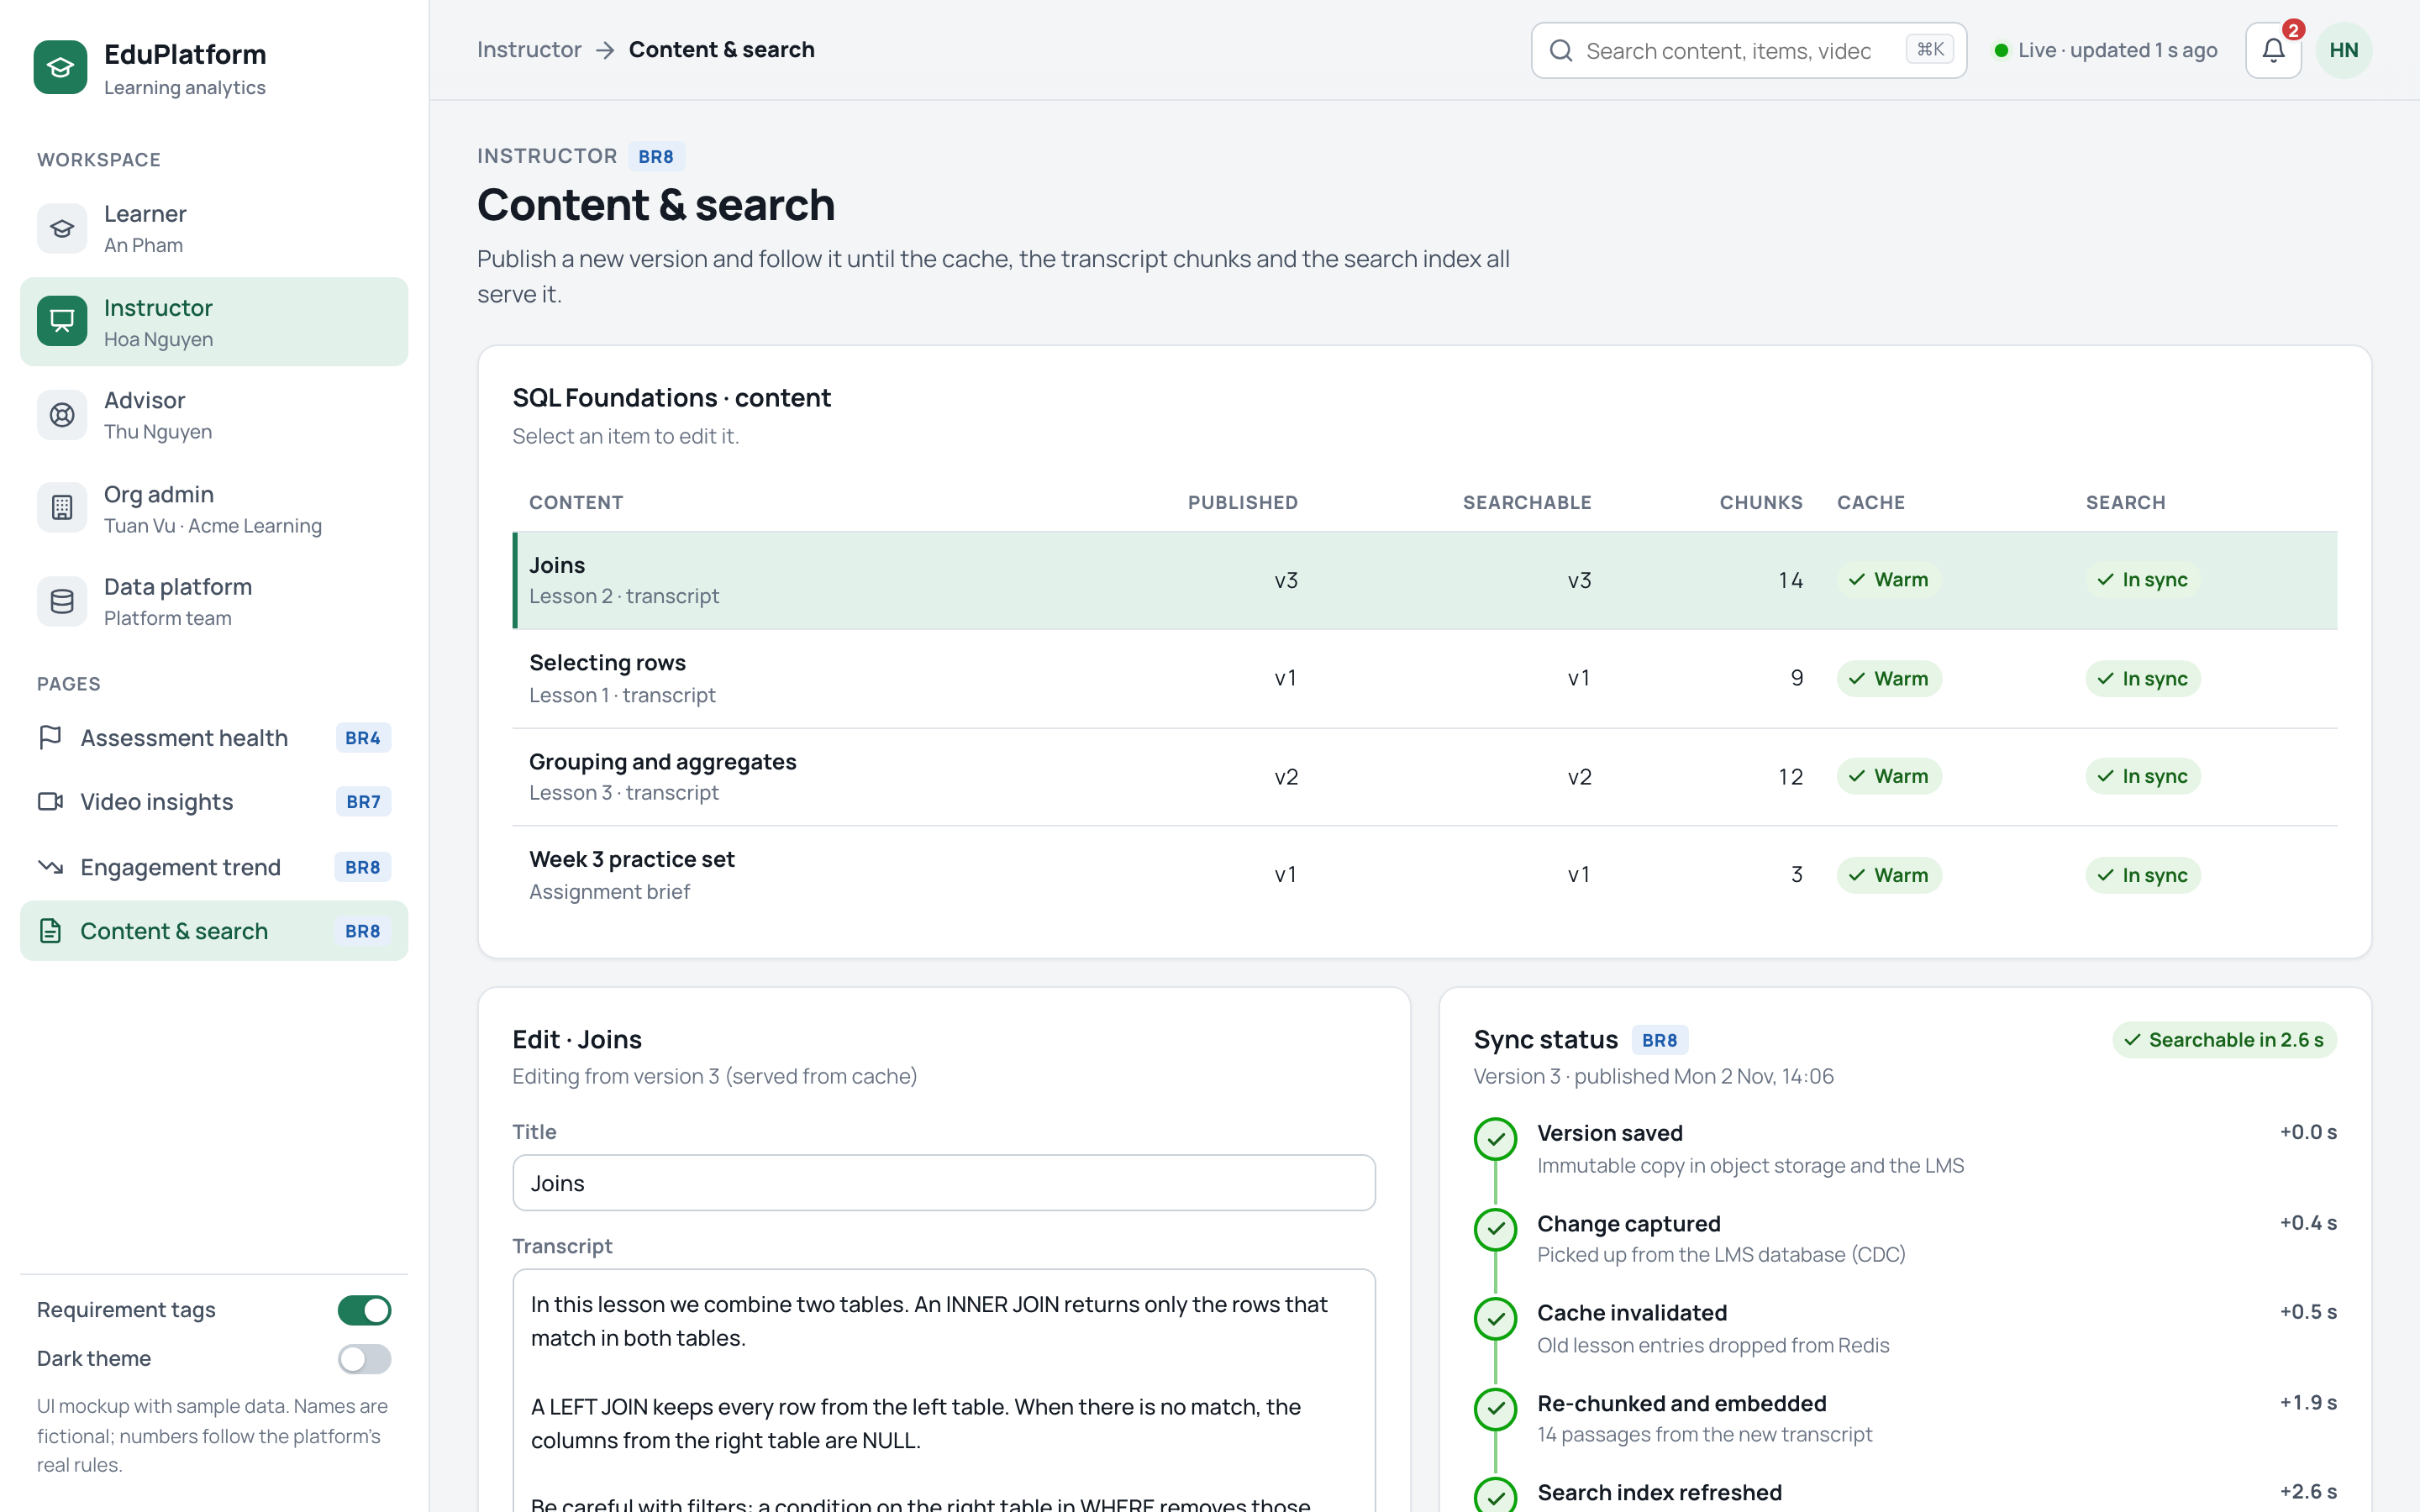
\includegraphics[width=\textwidth]{figures/mockup/instructor-content.png}
\caption{Mockup: Content \& search (BR8), theo dõi một phiên bản từ khi xuất bản đến khi tìm kiếm được}
\label{fig:mock-br8}
\end{figure}

\begin{figure}[H]
\centering
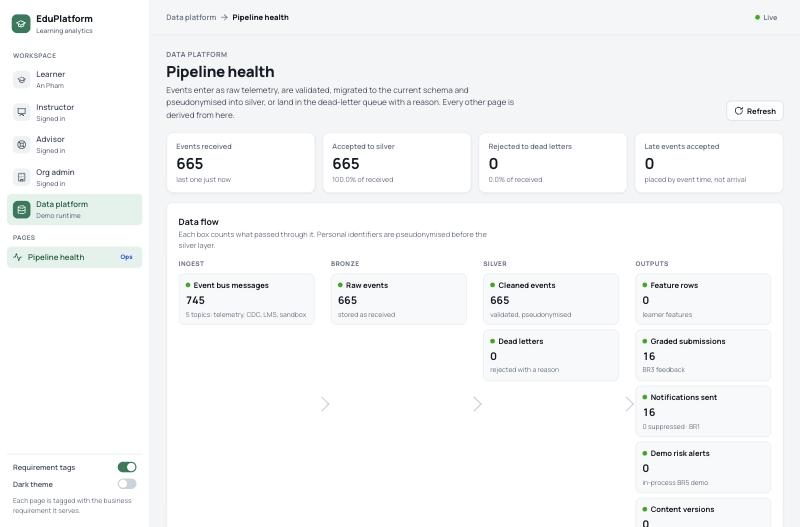
\includegraphics[width=\textwidth]{figures/ui/pipeline.jpg}
\caption{Pipeline health (chế độ sáng): bộ đếm của từng chặng trong luồng dữ liệu}
\label{fig:ui-pipeline}
\end{figure}

\begin{figure}[H]
\centering
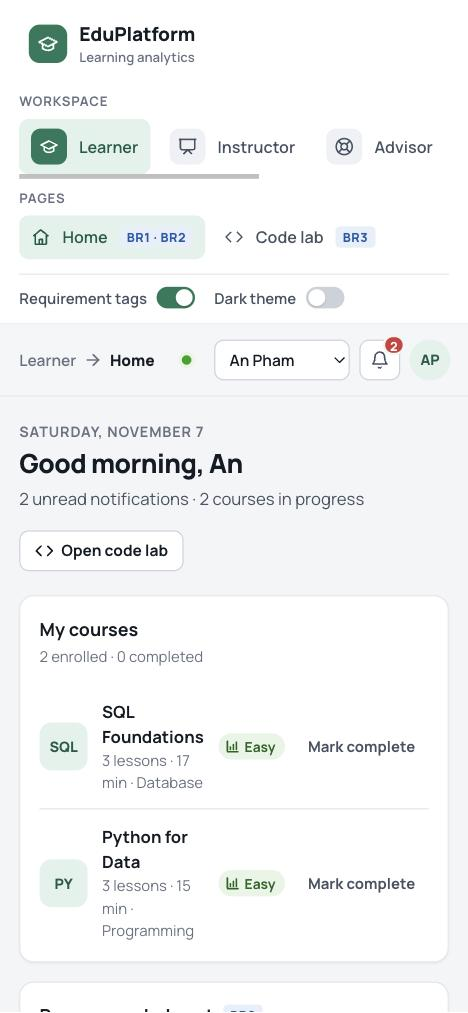
\includegraphics[width=0.42\textwidth]{figures/ui/learner-mobile.jpg}
\caption{Trang người học trên màn hình điện thoại (390 px): thanh bên chuyển thành tab ngang}
\label{fig:ui-mobile}
\end{figure}

\section{Kiểm thử giao diện}

Giao diện được kiểm chứng bằng ba cách:
\begin{itemize}
  \item \textbf{Biên dịch kiểu nghiêm ngặt}: TypeScript ở chế độ \code{strict}; bản build production thành công.
  \item \textbf{Kiểm tra thủ công trên trình duyệt} với dữ liệu thật ở chế độ sáng, tối, desktop và điện thoại. Một bài nộp thật đi qua sandbox và sinh ra một thông báo mới; các trang BR6--BR8 đọc mart thật từ Trino.
  \item \textbf{Kiểm thử chấp nhận bằng Playwright} (\code{apps/web/tests}), được cập nhật cho cấu trúc trang mới với các khẳng định nghiệp vụ giữ nguyên. Lần chạy sau khi thiết kế lại cho kết quả: ba test đạt (thông tin đăng nhập sai bị từ chối; báo cáo tổ chức ẩn nhóm nhỏ và chặn truy cập ngoài phạm vi; heatmap theo phiên bản và xu hướng tương tác). Các test còn lại cần những dịch vụ không chạy vào thời điểm đó (container \code{br45}, OpenSearch, lớp phủ trực tiếp) nên chưa được chạy lại trên giao diện mới.
\end{itemize}
